\section{模型评价}
\subsection{模型评价}
\subsubsection{模型优点}
\begin{enumerate}
\item 采用蒙特卡罗模拟的方法,通过在定日镜面和光锥内内生成随机光线,来模拟光线的入射和反射,省却了繁复的数学演算过程,降低了问题的建模难度。
\item 运用遗传算法求解决策变量和约束均较多情况下的单变量优化问题,并通过设置合适的种群数量、交叉变异概率、最大传代次数,提高算法的搜索能力,避免陷入局部最优。
\end{enumerate}

\subsubsection{模型缺点}
\begin{enumerate}
\item 计算阴影遮挡效率的算法运行时间较长,仍有改进优化的空间。 
\item 在问题2中设计镜场布局时,为了简化模型,只考虑了上文所描述的均匀布局,这种镜场设计可以满足单位面积输出热功率取最大值,但未考虑到实际应用中还应使得镜场总输出热功率尽可能大。
\end{enumerate}

\subsubsection{模型改进与推广}
在实际的镜场设计过程之中,可以叶序螺线(phyllotaxis spiral)布局,又称仿生布局(biomimetic layout)以及阿基米德螺线(Archimedean spiral)布局等\cite{noone},如下图所示:
\begin{figure}[H]
\centering
\begin{subfigure}[b]{0.4\textwidth}
\centering
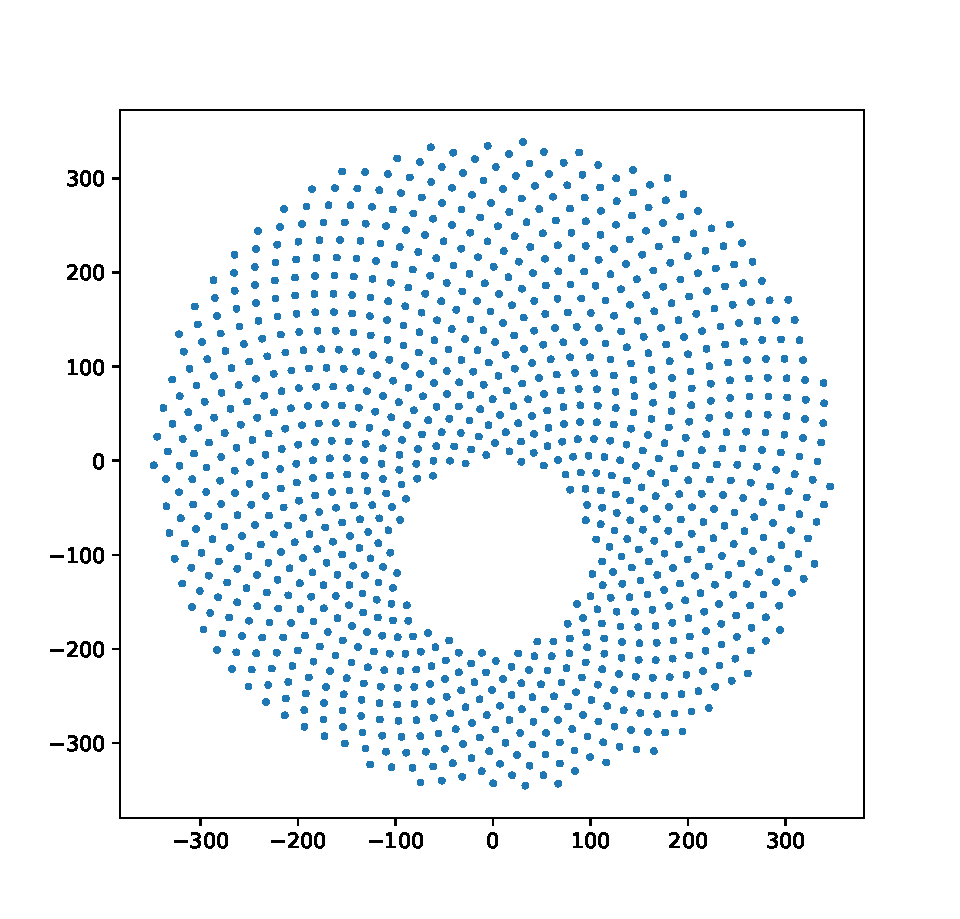
\includegraphics[scale=0.4]{yexu.pdf}
\caption{\kaishu 叶序螺线}
\end{subfigure}
%
\begin{subfigure}[b]{0.4\textwidth}
\centering
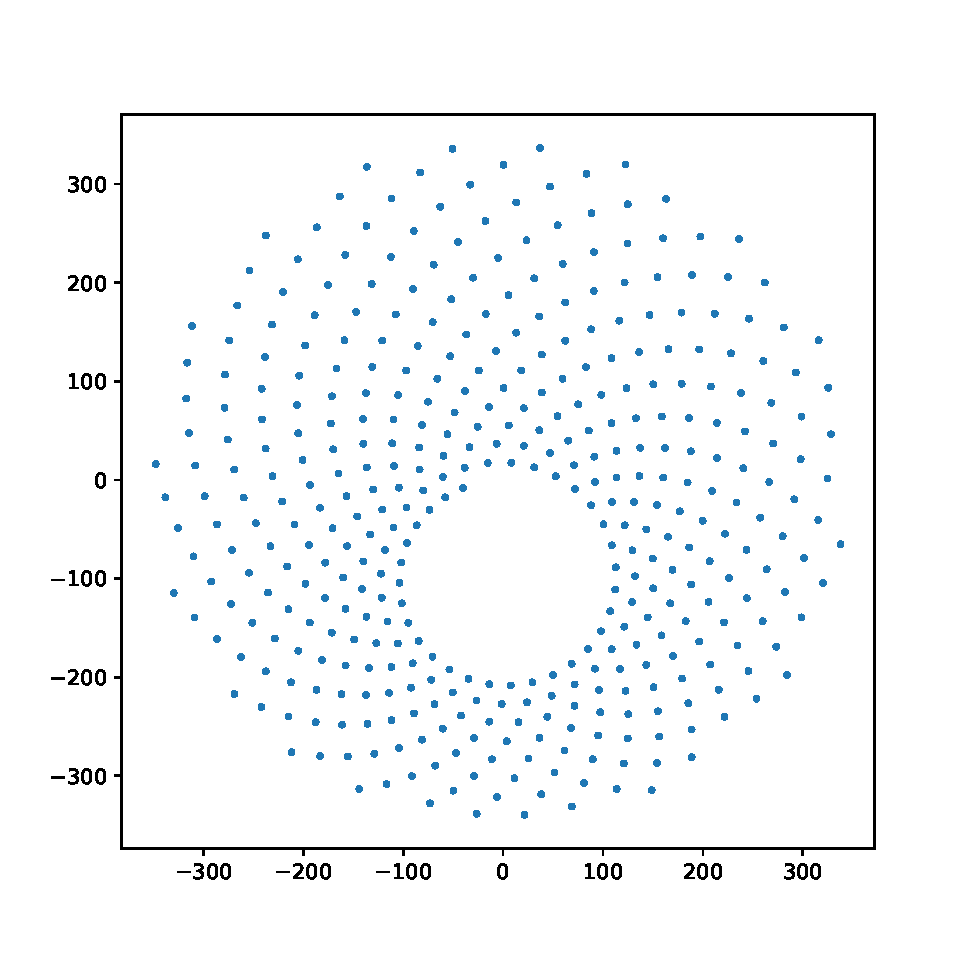
\includegraphics[scale=0.388]{ajmd.pdf}
\caption{\kaishu 阿基米德螺线}
\end{subfigure}
\end{figure}
